\documentclass[12pt]{report}
\usepackage{scrpage2}
\usepackage{graphicx}
\usepackage{caption}
\usepackage{subcaption}
\usepackage{acronym}
\usepackage{multirow}
\usepackage{parskip}
\usepackage{tikz}
\usetikzlibrary{arrows}
\usepackage{mdframed}
\usepackage{framed}
\usepackage{algorithm}
\usepackage{algpseudocode}
\usepackage{amsmath, amssymb, hyperref}
\graphicspath{{images/}}
\setcounter{secnumdepth}{3}
\setcounter{tocdepth}{4}

\title{
{Development of a Symbolic Model Checker}\\
{\large Institute of Electronic Design and Automation}\\
}
\author{Kasthuri Rengan Narayanan}
\date{Day Month Year}

\begin{document}
\maketitle
\tableofcontents
\chapter*{Abstract}
\thispagestyle{plain}
	Abstract goes here
Abstract goes here

\chapter*{List of Acronyms}
\begin{acronym}
\acro{BDD}{Binary Decision Diagram}
\acro{OBDD}{Ordered Binary Decision Diagram}
\acro{ROBDD}{Reduced Ordered Binary Decision Diagram}
\acro{LTL}{Linear Temporal Logic}
\acro{CTL}{Computational Tree Logic}
\acro{SAT}{Satisfiability}
\acro{CNF}{Conjunctive Normal Form}
\acro{DNF}{Disjunctive Normal Form}
\acro{POS}{Product of Sums}
\acro{SOP}{Sum Of Products}
\end{acronym}
\listoffigures
\listoftables
\chapter{Introduction}
The later half of the 20th century had seen a sea change in field of Integrated Circuits. The complexity of design had increased drastically from few hundred to billions of gates as of now. This made the conventional method of testing and simulation to be incomplete as one can never test the complete functionality of a system. This led to the idea of using Formal Verification in the field of Integrated Circuits."Formal verification is the act of proving or disproving the correctness of intended algorithms underlying a system with respect to a certain formal specification or property, using formal methods of mathematics"\cite{Alok 2010}. Formal verification provides exhaustive exploration of all possible behaviours rather than the traditional approach of simulation/testing which explore only few possible behaviours of a system. There are several methods of formal verification available out of which we will be looking into a method of model checking. The main advantages of the method is,
\begin{itemize}
\item The ability to perform verification in a completely automatic manner without any intervention from the user.
\item The result of model checking is always either True or False
\item If the property is failed to satisfy, it always produces a counterexample which provides an insight about the failure of the system
\end{itemize}

\chapter{Model Checking}
Model checking is the process of verifying the given model with the given set of specifications. The process of model checking involves
\begin{itemize}
\item Modelling
\item Specification
\item Verification
\end{itemize}

\begin{figure}[h]
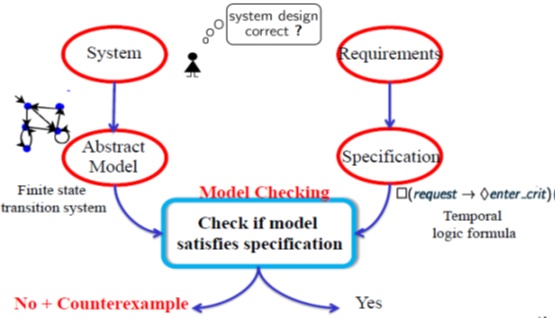
\includegraphics[scale=0.8]{model_checking}
\caption{Formal Verification using Model Checking}
\label{fig:sample_model_checking}
\end{figure}

Figure \ref{fig:sample_model_checking} shows the pictorial representation of Model checking.

Lets consider an example of a 2-bit counter with enable and reset and look how Formal verification using Model checking is done.\newline

\begin{figure}
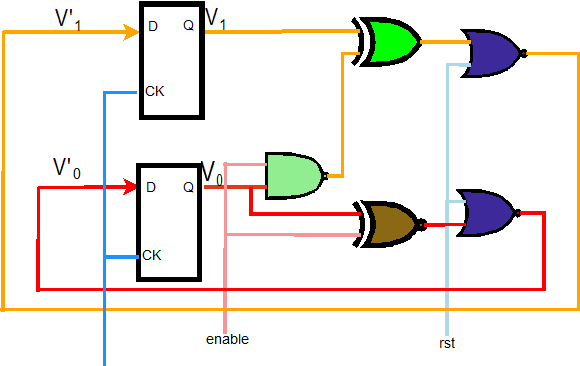
\includegraphics[scale=0.9]{counter_2}
\caption{Circuit of a 2-bit Counter}
\label{fig:2-bit Counter}
\end{figure}

Figure \ref{fig:2-bit Counter} is the circuit diagram of a 2-bit counter.

\begin{equation}
v0'\leftrightarrow\,\neg (rst\lor(\neg((enable\lor v0)\land(\neg enable\lor\neg v0)))
\label{eqn:v0}
\end{equation}
\begin{equation}
v1'\leftrightarrow \neg (rst\lor ((\neg enable\lor\neg v0)\lor v1)\land((v0\land enable)\lor \neg v1))
\label{eqn:v1}
\end{equation}

Equations \ref{eqn:v0} and \ref{eqn:v1} are the boolean expressions of the variable v0' and v1'. These equations are also called the transition relation of the variables. Equation \ref{eqn:v0} corresponds to transition relation of variable v0 and equation \ref{eqn:v1} corresponds to transition relation of variable v1. For simplicity lets assume enable is always True. Now the equations becomes

\begin{equation}
v0'\leftrightarrow\,\neg (rst\lor v0)
\label{eqn:v0_1}
\end{equation}
\begin{equation}
v1'\leftrightarrow \neg (rst\lor ((\neg v0 \lor v1)\land(v0 \lor \neg v1)))
\label{eqn:v1_1}
\end{equation}

\section{Model}
The first step in model checking is to generate a model for the system. Model should capture all the properties of the system. The most important feature of a system is its state. State is the snapshot of the values of the variables of a system at a particular instant of time. State upon which an action is performed results in a new state. Pair of such states determines the transition of the system. To capture these behaviours of a system, we use kripke structure, a state transition graph.
\subsection{Kripke Structure}
We use Kripke structure for modelling our system. Kripke structure is a tuple M = (S,R,I,AP,L).
\begin{itemize}
\item $S$ is set of states
\item $R\subseteq S\times S$ is the transition relation
\item $I\subseteq S$ is the set of possible initial states
\item $AP$ is a set of atomic propositions
\item $L:S\rightarrow 2^{AP}$ is a labeling function: each state is labeled with the\\ atomic propositions that are true in that state
\end{itemize}
S is also called as the state space of the system.
\newline

\begin{figure}
\centering
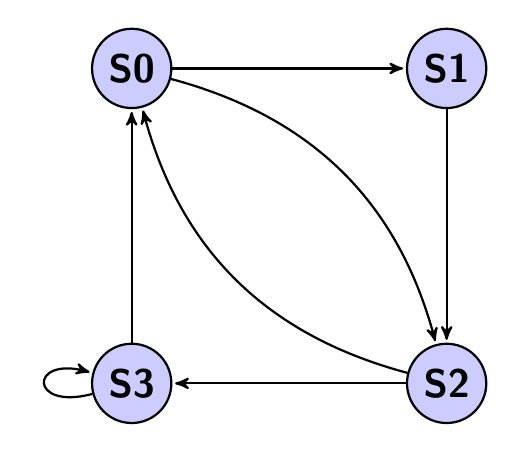
\begin{tikzpicture}[->,>=stealth',shorten >=1pt,auto,node distance=4cm,
  thick,main node/.style={circle,fill=blue!20,draw,font=\sffamily\Large\bfseries}]

  \node[main node] (1)  {S0};
  \node[main node] (2) [right of=1] {S1};
  \node[main node] (3) [below of=2] {S2};
  \node[main node] (4) [below of=1] {S3};

  \path[every node/.style={font=\sffamily\small}]
    (1) edge (2)
        edge [bend left] (3)
    (2) edge (3)
    (3) edge (4)
        edge [bend left] (1)
    (4) edge (1)
         edge[loop left] (4)
         ;
\end{tikzpicture}
\caption{Kripke structure} \label{kripke structure}
\end{figure}


The Figure ~\ref{kripke structure} is a kripke structure. S0,S1,S2 and S3 are the states of the system. \{S0,S1\},\{S0,S2\},\{S3,S3\}.. are the transitions of the system.
\newline

Till early 1980's, transition relation of a system was represented using adjacency list\cite{Clarke 2008}.  Due to the increase in the number of states, state transition graph became too large to handle using adjacency list. \cite{McMillian 1993} suggested a novel approach to solve the state exploration problem by using a symbolic representation of the state transition graph. It was based on ROBDD. For a given order, ROBDD of a boolean expression is always canonical\cite{Bryant 1986}.
\subsection{Binary Decision Diagram}
Boolean expressions can be represented using a rooted, direct, acyclic graph called the BDD. BDD was first introduced by Lee\cite{Lee,1959}. An efficient data structure for representing the BDD and efficient algorithms for manipulating BDD's were later developed by \cite{Bryant 1986}. He also introduced the concept of ordering of variables in a BDD, which would affect the size significantly. 

Let's see few important expressions for BDD manipulations.

\subsubsection*{Shannon Expansion}
It is defined as the expansion of a boolean formula with respect to a boolean variable. $f|_{x\leftarrow 0}$ and $f|_{x_\leftarrow 1}$ are called the positive and negative Shannon co-factors of  boolean formula f with respect to boolean variable x.
\begin{equation}
\label{shannon}
f=(\neg x\land f|_{x\leftarrow 0}) \lor (x\land f|_{x\leftarrow 1})
\end{equation}

\subsubsection*{Existential quantification}
If either the positive co-factor or the negative co-factor of a boolean expression with respect to a boolean variable x is true, then the boolean variable x can be existentially quantified out.
\begin{equation}
\label{eqn:EQ}
\exists_xf=f|_{x\leftarrow 0} \lor f|_{x\leftarrow 1}
\end{equation}


\subsubsection*{Universal quantification}
Only if both the positive and negative co-factor of a boolean expression with respect to a boolean variable x is true, then the boolean variable x can be universally quantified out. 
\begin{equation}
\label{UQ}
\forall_xf=f|_{x\leftarrow 0} \land f|_{x\leftarrow 1}
\end{equation}

\subsubsection*{BDD Operations}
Boolean operations like AND, OR, NOT etc.. can be implemented as algorithms on OBDD's. The algorithm takes OBDD's as input and produce a reduced form of OBDD's\cite{Bryant 1986}. The variable ordering of the original OBDD's are preserved. The reduction of OBDD is based on the following reduction rules.

\begin{itemize}
\item Any node having identical child nodes are removed.
\item 2 Nodes with isomorphic BDD's are removed.
\end{itemize}

ROBDD is the most compact representation of BDD by using the above mentioned reduction rule which results in eliminating nodes which in turn reduces the memory used to construct ROBDD. 
\begin{equation}
f<op>g = (\neg x \land (f|_{x\leftarrow 0} <op> g|_{x\leftarrow 0})) \lor (x \land (f|_{x\leftarrow 1} <op> g|_{x\leftarrow 1}))
\label{eqn:op}
\end{equation}

Equation ~\ref{eqn:op} can be recursively called for computing the OBDD representation of $f<op>g$. Reduction rules can be applied alongside the operation thereby generating a ROBDD.
\subsection{Representing Kripke structure using BDD}
\label{sec:model_bdd}
We have already seen how ROBDD is useful in compact representation of a boolean expression. McMillan suggested a novel approach in the field of model checking by using ROBDD's for the symbolic representation of state transition graphs \cite{Burch 1990}\cite{McMillan 1993}.

Lets now look with an example how kripke structure can be represented using ROBDD. Consider the kripke structure in the figure \ref{fig:kripke structure 2-bit counter}. There are 3 state variables v1,v0 and rst. 3 additional state variables v1',v0' and rst' are introduced to encode the successor states. v1,v0 and rst are the present state variables while v1',v0' and rst' are the next state variables.

Table \ref{table:state_encoding} shows the state encoding table of the figure \ref{fig:kripke structure 2-bit counter}. Only the transition relations present in figure \ref{fig:kripke structure 2-bit counter} are considered in the table \ref{table:state_encoding}. Thus the transition from state 000 to state 010 in figure \ref{fig:kripke structure 2-bit counter} is represented in first row in table \ref{table:state_encoding} which can be written as $\neg v1 \land \neg v0 \land \neg rst \land \neg v1' \land v0' \land \neg rst'$. In the same way second transition in table \ref{table:state_encoding} can be written as $\neg v1 \land \neg v0 \land \neg rst \land \neg v1' \land v0' \land rst'$. Similarly all the transitions in state transition graph can be encoded. The transition relation of the system can be obtained by the disjunction of all the rows in state encoding table \ref{table:state_encoding}.

$(\neg v1 \land \neg v0 \land \neg rst \land \neg v1' \land v0' \land \neg rst') \lor (\neg v1 \land \neg v0 \land \neg rst \land \neg v1' \land v0' \land rst') \lor ...$


\begin{table}[H]
\centering
\begin{tabular}{ |c|c|c|c|c|c| }
\hline
\multicolumn{3}{|c|}{Present state} & \multicolumn{3}{|c|}{Next state}\\
\hline
v1 & v0 & rst & v0' & v1' & rst'\\
\hline
& & & 0 & 1 & 0 \\[-1ex]
\raisebox{1.5ex}{0} & \raisebox{1.5ex}{0} & \raisebox{1.5ex}{0} & 0 & 1 & 1\\
\hline
& & & 0 & 0 & 0\\[-1ex]
\raisebox{1.5ex}{0} & \raisebox{1.5ex}{0} & \raisebox{1.5ex}{1} & 0 & 0 & 1\\
\hline
& & & 1 & 0 & 0\\[-1ex]
\raisebox{1.5ex}{0} & \raisebox{1.5ex}{1} & \raisebox{1.5ex}{0} & 1 & 0 & 1\\
\hline
& & & 0 & 0 & 0\\[-1ex]
\raisebox{1.5ex}{0} & \raisebox{1.5ex}{1} & \raisebox{1.5ex}{1} & 0 & 0 & 1\\
\hline
& & & 1 & 1 & 1\\[-1ex]
\raisebox{1.5ex}{1} & \raisebox{1.5ex}{0} & \raisebox{1.5ex}{0} & 1 & 1 & 0\\
\hline
& & & 0 & 0 & 0\\[-1ex]
\raisebox{1.5ex}{1} & \raisebox{1.5ex}{0} & \raisebox{1.5ex}{1} & 0 & 0 & 1\\
\hline
& & & 0 & 0 & 0\\[-1ex]
\raisebox{1.5ex}{1} & \raisebox{1.5ex}{1} & \raisebox{1.5ex}{0} & 0 & 0 & 1\\
\hline
& & & 0 & 0 & 0\\[-1ex]
\raisebox{1.5ex}{1} & \raisebox{1.5ex}{1} & \raisebox{1.5ex}{1} & 0 & 0 & 1\\
\hline
\end{tabular} 
\caption{State Encoding for 2-bit Counter}
\label{table:state_encoding}
\end{table}

The transition relation is then converted to an ROBDD for a compact representation. Figure \ref{fig:ROBDD_counter} shows the ROBDD representation of the transition relation of 2-bit counter. In most of the cases encoding the transition relation as mentioned above from the kripke structure is not feasible as the state transition graph is too large. So, ROBDD is generated from the high-level description of the system. From the equation \label{eqn:v0_0} and \label{eqn:v0_1} transition relation of the whole system can be built. The transition relation of a system is the conjunction of the transition relation of individual variables.
\begin{equation}
(v0'\leftrightarrow\,\neg (rst\lor v0)) \land (v1'\leftrightarrow \neg (rst\lor ((\neg v0 \lor v1)\land(v0 \lor \neg v1)))
\label{eqn:TR}
\end{equation}
Equation \ref{eqn:TR} is the transition relation of the system.

\begin{figure}[H]
\centering
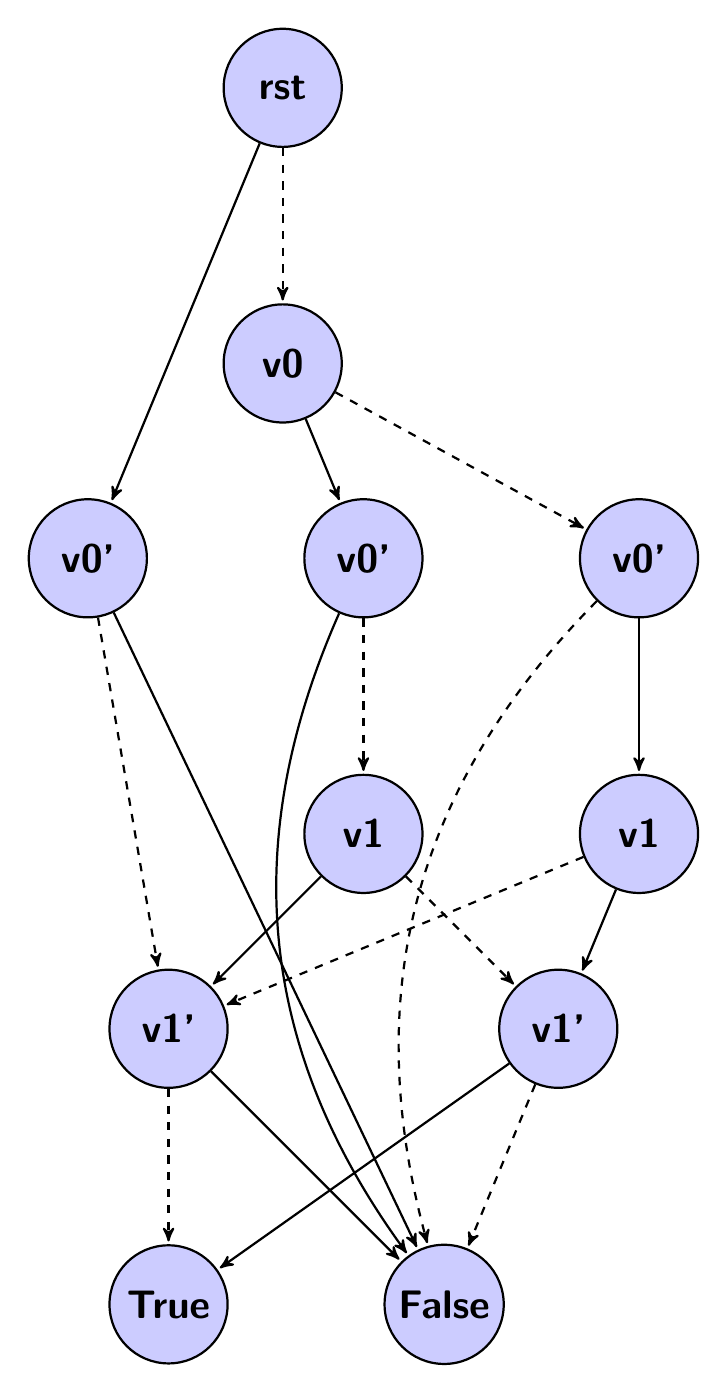
\begin{tikzpicture}[->,>=stealth',shorten >=1pt,node distance=3.5cm,
  thick,main node/.style={circle,fill=blue!20,draw,font=\sffamily\Large\bfseries,minimum size=1.5cm}]

  \node[main node] (2) {rst};
  \node[main node] (4) [below of=2] {v0};
  \node[main node] (6) [below left of=4] {v0'};
  \node[main node] (7) [right of=6] {v0'};
  \node[main node] (8) [right of=7] {v0'};
  \node[main node] (10) [below of=7] {v1};
  \node[main node] (11) [right of=10] {v1};

  \node[main node] (12) [below left of=10] {v1'};
  \node[main node] (13) [below right of=10] {v1'};
  \node[rectangle,main node] (14) [below of=12] {True};
\node[rectangle,main node] (15) [right of=14] {False};


  \path[every node/.style={font=\sffamily\small}]
     (2) edge (6)
          edge[dashed](4)
     (4)edge(7)
          edge[dashed](8)
    (6)edge(15)   
         edge[dashed](12)
   (7)edge[bend right](15)
       edge[dashed](10)
    (8)edge(11)
        edge[bend right,dashed](15)
   (10)edge(12)
         edge[dashed](13)
   (11)edge(13)
         edge[dashed](12)
   (12)edge(15)
         edge[dashed](14)
   (13)edge(14)
          edge[dashed](15)
     

;
\end{tikzpicture}
\caption{ROBDD representation of transition relation of 2-bit counter}
\label{fig:ROBDD_counter}
\end{figure}

\section{Specification}
\label{sec:specification}
\begin{itemize}
\item Does a program reach a state in future?
\item Will the program eventually terminate?
\item Does the program always behave correctly?
\end{itemize}

For specifying such properties we need "Temporal Logic". 

\subsection{Temporal Logic}
It expresses the ordering of events in time. It is the formalism for describing transitions in a reactive system. In temporal logic, time is not explicitly mentioned rather mentioned like eventually a state will be reached or never error state is reached. Temporal logic basically has 2 kinds of operators. They are logical operators like AND,OR,NOT, IMPLICATION etc.. and modal operators like X, F, G etc... Temporal logic can be differentiated into 2 kinds namely linear and branching time logic. In linear time logic, events along a single computational path are described. In branching time logic, events along the paths from a state are described.

Liner temporal logic(LTL) is a linear time logic and Computational Tree Logic (CTL) is a branching time logic. Combination of both LTL and CTL is CTL*, which is the most powerful temporal logic.In our tool we have used only CTL. In this report, only CTL will be discussed. CTL formulas are composed of path quantifiers and temporal operators. 

\subsubsection*{Path quantifiers:}
Branching structure in a computation tree is described using path quantifier. There are 2 path quantifiers\cite{Clarke 1999}
\begin{itemize}
\item A : For ALL computation paths
\item E : For some computation path
\end{itemize}
In a state, these quantifiers are used by specifying all the paths or along some paths some property holds from that state.

\subsubsection*{Temporal Operators:}
Properties of a path in a computation tree is described by temporal operators. There are basically 4 temporal operators
\begin{itemize}
\item X "Next" - Property holds in the second state of the path.
\item F "Future" - Property will hold at some state along the path.
\item G "Global" - Property holds at every state along the path.
\item U "Until" (f U g) - Property g holds in some states until then property f holds along the path.
\end{itemize}

There are 2 types of formulas in Temporal Logic.

\subsubsection*{State Formula:}
\begin{itemize}
\item It is defined as the formula which holds true in a specific state.
\item If $p\in AP$, then p is a state formula.
\item If f and g are state formulas, then $\neg f, f\lor g,f\land g$ are also state formulas.
\item If f is a path formula, then E f and A f are state formulas.
\end{itemize}

\subsubsection*{Path Formula:}
\begin{itemize}
\item It is defined as the formula which holds true along a specific path.
\item if f and g are path formulas, then $\neg f, f\lor g,f\land g, X f,F f,G f,f U g$ are also path formulas.
\end{itemize}

CTL uses only state formulas. In CTL, temporal operators should always be preceded by a path quantifier.

\subsubsection*{Syntax of CTL:}
CTL formula are always formed according to the following grammar.

\begin{center}
$\phi::=true\mid a\mid \phi_1\wedge\phi_2\mid\neg\phi\mid E \psi\mid\forall\psi$
\end{center}

where $a\in AP$ and $\psi$ is a path formula and also a temporal operator. CTL  path formula are formed according to following grammar.

\begin{center}
$\psi::=X\phi\mid\phi_1\cup\phi_2$
\end{center}

where $\phi_1$ and $\phi_2$ are state formula.

\subsubsection*{CTL operators:}
There are 8 basic CTL operators. 
\begin{itemize}
\item AX and EX
\item AF and EF
\item AG and EG
\item AU and EU
\end{itemize}

3 main operators used in our tool are EX, EG and EU. All the remaining operators can be expressed using the above mentioned 3 operators.

\begin{itemize}
\item AX f = $\neg E X(\neg f)$
\item EF f = $E (True U f)$
\item AF f = $\neg E G(\neg f)$
\item AG f = $\neg E F(\neg f)$
\item A(f U g) = $\neg E(\neg g U (\neg f \land \neg g)) \land \neg E G\neg g$
\end{itemize}

\begin{figure}[H]
\begin{tabular}{c  c}
\begin{subfigure}{.5\textwidth}
\centering
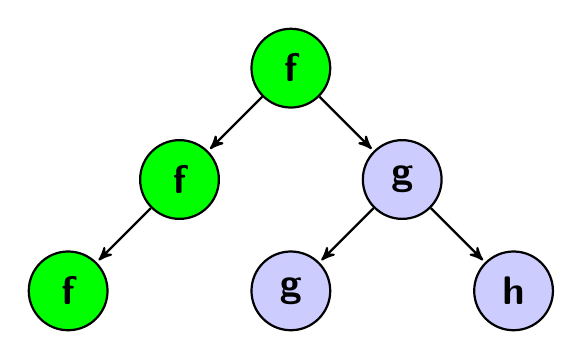
\begin{tikzpicture}[->,>=stealth',shorten >=1pt,node distance=2cm,
  thick,main node/.style={circle,fill=blue!20,draw,font=\sffamily\Large\bfseries,minimum size=1cm}]

  \node[main node,fill = green] (0) {f};
  \node[main node,fill = green] (1) [below left of=0] {f};
  \node[main node] (2) [below right of=0] {g};
  \node[main node,fill = green] (3) [below left of=1] {f};
  \node[main node] (4) [below right of=2] {h};
  \node[main node] (5) [below left of=2] {g};
  
    \path[every node/.style={font=\sffamily\small}]
     (0) edge (1)
          edge (2)
     (1)edge (3)
    (2)edge(4)   
         edge(5)
;
\end{tikzpicture}
\caption{E G f}
\label{E G f}
\end{subfigure}
\hfill\hfill\hfill
&
\begin{subfigure}{.5\textwidth}
\centering
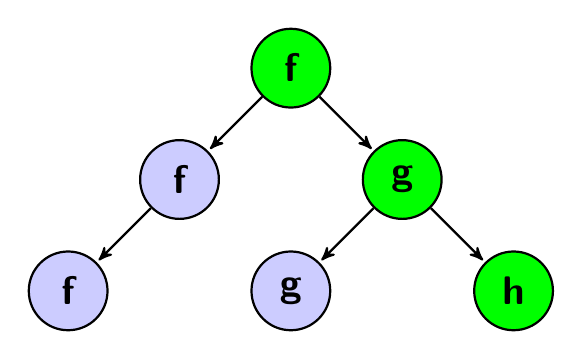
\begin{tikzpicture}[->,>=stealth',shorten >=1pt,node distance=2cm,
  thick,main node/.style={circle,fill=blue!20,draw,font=\sffamily\Large\bfseries,minimum size=1cm}]

  \node[main node,fill = green] (0) {f};
  \node[main node] (1) [below left of=0] {f};
  \node[main node,fill = green] (2) [below right of=0] {g};
  \node[main node] (3) [below left of=1] {f};
  \node[main node,fill = green] (4) [below right of=2] {h};
  \node[main node] (5) [below left of=2] {g};
  
    \path[every node/.style={font=\sffamily\small}]
     (0) edge (1)
          edge (2)
     (1)edge (3)
    (2)edge(4)   
         edge(5)
;
\end{tikzpicture}
\caption{E F h}
\label{E F h}
\end{subfigure}

\\
\\
\begin{subfigure}{.5\textwidth}
\centering
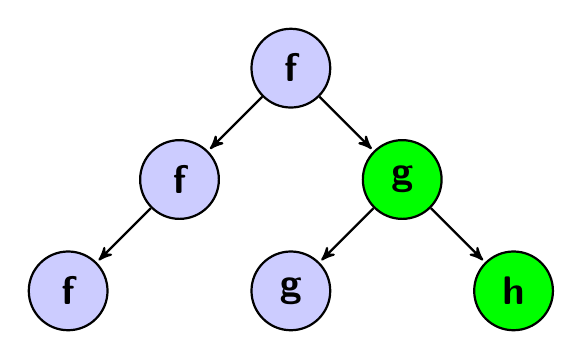
\begin{tikzpicture}[->,>=stealth',shorten >=1pt,node distance=2cm,
  thick,main node/.style={circle,fill=blue!20,draw,font=\sffamily\Large\bfseries,minimum size=1cm}]

  \node[main node] (0) {f};
  \node[main node] (1) [below left of=0] {f};
  \node[main node,fill = green] (2) [below right of=0] {g};
  \node[main node] (3) [below left of=1] {f};
  \node[main node,fill = green] (4) [below right of=2] {h};
  \node[main node] (5) [below left of=2] {g};
  
    \path[every node/.style={font=\sffamily\small}]
     (0) edge (1)
          edge (2)
     (1)edge (3)
    (2)edge(4)   
         edge(5)
;
\end{tikzpicture}
\caption{E (g U h)}
\label{E (g U h)}
\end{subfigure}
\hfill\hfill\hfill
&
\begin{subfigure}{.5\textwidth}
\centering
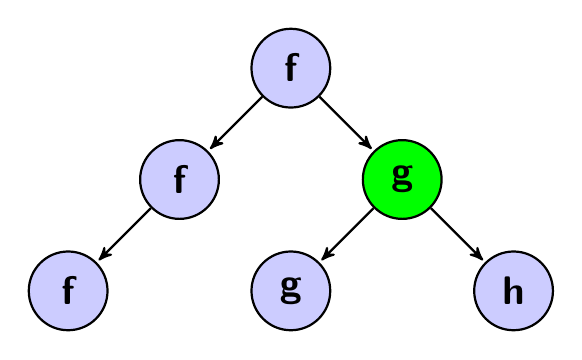
\begin{tikzpicture}[->,>=stealth',shorten >=1pt,node distance=2cm,
  thick,main node/.style={circle,fill=blue!20,draw,font=\sffamily\Large\bfseries,minimum size=1cm}]

  \node[main node] (0) {f};
  \node[main node] (1) [below left of=0] {f};
  \node[main node,fill = green] (2) [below right of=0] {g};
  \node[main node] (3) [below left of=1] {f};
  \node[main node] (4) [below right of=2] {h};
  \node[main node] (5) [below left of=2] {g};
  
    \path[every node/.style={font=\sffamily\small}]
     (0) edge (1)
          edge (2)
     (1)edge (3)
    (2)edge(4)   
         edge(5)
;
\end{tikzpicture}
\caption{E X h}
\label{E X h)}
\end{subfigure}
\\
\end{tabular}
\caption{Basic CTL operators}
\label{fig:basic ctl operators}
\end{figure}

Figure ~\ref{fig:basic ctl operators} shows the pictorial representation of few basic CTL operators.

\section{Verification}
In section ~\ref{sec:model_bdd} we have discussed how ROBDD is used to represent the model of the system. To verify the model using the specification we need algorithms that operates on ROBDD. In this section we will be seeing few basic CTL model checking algorithms which are used to verify the ROBDD model with the CTL specification. As mentioned in section ~\ref{sec:specification}, we will be looking into algorithms of 3 basic CTL operators used in our tool E X, E G, E U.

\subsection*{Symbolic computation of E X}
Equation ~\ref{eqn:exists_next} is the symbolic computation algorithm for E X $\Phi$. It is a straightforward procedure where E X $\Phi$ is true in a state, if in the successor state $\Phi$ is true.

\begin{equation}
\label{eqn:exists_next}
EX(\Phi)\,=\,[EX(\Phi)](V)\,=\,\exists_{V'} [N(V,V')\wedge \Phi(V')]
\end{equation}

$N(V,V')$ is the ROBDD representation of transition relation of the system. $\Phi(V')$ is the ROBDD representation of the given CTL expression. Once we have both the ROBDD's we can find E X using the equation ~\ref{eqn:EQ}.

\subsection*{Relational Product Computation}

From equation ~\ref{eqn:exists_next} one can easily compute E X by using an BDD AND operation on ROBDD's $\Phi(V')$ and $N(V,V')$ and then applying existential quantification using equation ~\ref{eqn:EQ}. As seen in figure ~\ref{fig:ROBDD_counter}, ROBDD representation of a transition relation contains both present state and next state variables. We use existential quantification to quantify out next state variables. The ROBDD of $N(V,V') \land \Phi(V')$ will always be much larger than the final result. A new algorithm was proposed to compute the resultant ROBDD by performing AND operation and existential quantification in a single step \cite{Clarke 1999}. Figure ~\ref{Relational Product algorithm} shows the algorithm for computing relational product.

f and g are the 2 ROBDD's representing transition relation and CTL expression. E contains the set of variables which are to be existentially quantified out. In figure ~\ref{Relational Product algorithm} line 2-5 corresponds to basic AND operation while line 15 corresponds to existential quantification. 

\begin{figure}[H]
\begin{framed}
\begin{algorithmic}[1]
\Procedure{RelProd}{$f,$g:BDD,$E:set\_of\_variables$}$:BDD$
\If{$f = false \lor g = false$}
 \State $return$ $false$
\ElsIf{$f = true \land g = true$}
 \State $return$ $true$
\ElsIf{$(f,g,E,h)$ $in$ $result$ $cache$}
 \State $return$ $h$
\Else
 \State $let$ $x$ $be$ $the$ $top$ $variable$ $of$ f
 \State $let$ $y$ $be$ $the$ $top$ $variable$ $of$ g
 \State $let$ $z$ $be$ $the$ $topmost$  $of$ $f$ and g
 \State {$h_0 = RelProd(f\mid_{z\to 0},g\mid_{z\to 0},E)$}
 \State {$h_1 = RelProd(f\mid_{z\to 1},g\mid_{z\to 1},E)$}
 \If{$z\in E$}
  \State {$h = OR(h_0,h_1)$} //$BDD for h_0 \lor h_1$
 \Else
  \State {$h=IfThenElse(z,h_0,h_1)$}
  \State $      /*BDD for (z\land h_1) \lor (\neg z\land h_0)*/$
 \EndIf
 \State {$insert(f,g,E,h)in$} result cache
 \State return h
\EndIf
\EndProcedure
\end{algorithmic}
\end{framed}
\caption{Relational Product algorithm}
\label{Relational Product algorithm}
\end{figure}

\subsection*{Symbolic computation of E U}

Figure ~\ref{Symbolic computation of E U} shows the algorithm for symbolic computation of $E (\Phi 1 U \Phi 2)$ CTL operator \cite{Baier 2008}.   

\begin{figure}[H]
\begin{framed}
\begin{algorithmic}[1]
\Procedure{symbolic computation of}{$ E(\phi 1\, U\, \phi 2)$}
\State $f_0(V) = \chi_{\phi 2}(V)$
\State $j = 0$
\Repeat
\State $f_{j+1}(V) = f_j(V) \lor (\chi_{\phi 1} \land \exists_{V'}[N(V,V')\land f_j(V')]);$
\State j = j+1;
\Until  $f_j(V) = f_{j-1}(V);$
\State
\Return $f_j(V)$

\EndProcedure
\end{algorithmic}
\end{framed}
\caption{Symbolic computation of E U}
\label{Symbolic computation of E U}
\end{figure}


\subsection*{Symbolic computation of E G}

Figure ~\ref{Symbolic computation of E G} shows the algorithm for symbolic computation of $E G(\Phi 1)$ CTL operator \cite{Baier 2008}. 

\begin{figure}[H]
\begin{framed}
\begin{algorithmic}[1]
\Procedure{symbolic computation of}{$ E G(\phi 1)$}
\State $f_0(V) = \chi_{\phi 1}(V)$
\State $j = 0$
\Repeat
\State $f_{j+1}(V) = f_j(V) \land (\chi_{\phi 1} \land \exists_{V'}[N(V,V')\land f_j(V')]);$
\State j = j+1;
\Until  $f_j(V) = f_{j-1}(V);$
\State
\Return $f_j(V)$

\EndProcedure
\end{algorithmic}
\end{framed}
\caption{Symbolic computation of E G}
\label{Symbolic computation of E G}
\end{figure}




\chapter{Partitioned Transition Relation}
kdbhajfb

\chapter{Cone Of Influence Reduction}
efewf

\chapter{SAT Solver}
rfnefl


\begin{thebibliography}{99}
\bibitem{Alok 2010} Alok Sanghavi \emph{What is formal verification?} 21 May 2010: EE Times\_Asia.
\bibitem{Clarke 2008} Edmund M Clarke\emph{The Birth of Model checking} 25 years of model checking,2008.
\bibitem{McMillan 1993} Kenneth L McMillan\emph{Symbolic Model Checking: An approach to the State Explosion Problem} kluwer Academic Publishers,1993.
\bibitem{Burch 1990} J.R. Burch, E.M. Clarke, K.L. McMillan,D.L. Dill and J. Hwang. \emph{Symbolic Model Checking:10\textsuperscript{20} states and beyond.} In proc. 5th Ann.Symp. on Logic in Computer Science. IEEE comp.Soc.Press, June 1990.
\bibitem{Bryant 1986} Randal E Bryant\emph{Graph-Based Algorithms for Boolean Function Manipulation} IEEE Transactions on Computers C-35-8:677-691, August 1986
\bibitem{Lee 1959} C.Y.Lee \emph{Binary decision programs} Bell System Technical Journal.38(4):985-999, July 1959.
\bibitem{Bryant 1992} Randal E Bryant\emph{Symbolic Boolean Manipulation with Ordered Binary Decision Diagrams} ACM Computing Surveys,1992
\bibitem{Clarke 1999}Edmund M. Clarke,Orna Grumberg, Doron A. Peled \emph{Model Checking} ISBN 0-262-03270-8,1999
\bibitem{Baier 2008} Christel Baier, Joost-Pieter Katoen \emph{Principles of model checking} ISBN 978-0-262-02649-9
\end{thebibliography}

\end{document}